\documentclass[11pt]{beamer}
\usetheme{Boadilla}
\usepackage[utf8]{inputenc}
\usepackage[czech]{babel}
\usepackage[T1]{fontenc}
\usepackage{amsmath}
\usepackage{amsfonts}
\usepackage{amssymb}
\usepackage{amsthm}
\usepackage{graphicx}
\usepackage{datetime}

\author{Jan Tušil}

\newdate{date}{19}{06}{2015}
\date{\displaydate{date}}

\title{Partial Order Reduction pro LLVM IR}
%\setbeamercovered{transparent} 
%\setbeamertemplate{navigation symbols}{} 
%\logo{} 
%\institute{} 
\date{\displaydate{date}} 
\subject{Obhajoba bakalářské práce}

\begin{document}

%\begin{frame}
%\titlepage
%\end{frame}

%\begin{frame}
%\tableofcontents
%\end{frame}

\newtheorem{question}{Otázka}

\begin{frame}{Cíl práce}
Redukce stavového prostoru
paralelních programů.
%s cílem urychlit verifikaci.
\begin{itemize}
\item Vstup: program v jazyce LLVM IR + Posix Threads
\item Výstup: přechodový systém v jazyce NTS
\item Technika: redukce částečným uspořádáním (POR)
\end{itemize}
\end{frame}

\begin{frame}{LLVM IR}
\begin{figure}
\includegraphics[scale=0.4]{LLVMCompiler1.png}
\caption{Použití LLVM\footnote{Zdroj obrázku: http://www.aosabook.org/en/llvm.html}}
\end{figure}
\begin{itemize}
\item LLVM - framework pro tvorbů překladačů
\item LLVM IR - Jazyk pro mezikód ve stylu assembleru
\item LLVM IR = assembler (RISC) + typy + funkce
\end{itemize}
\end{frame}

\begin{frame}{Přechodové systémy}
\begin{figure}
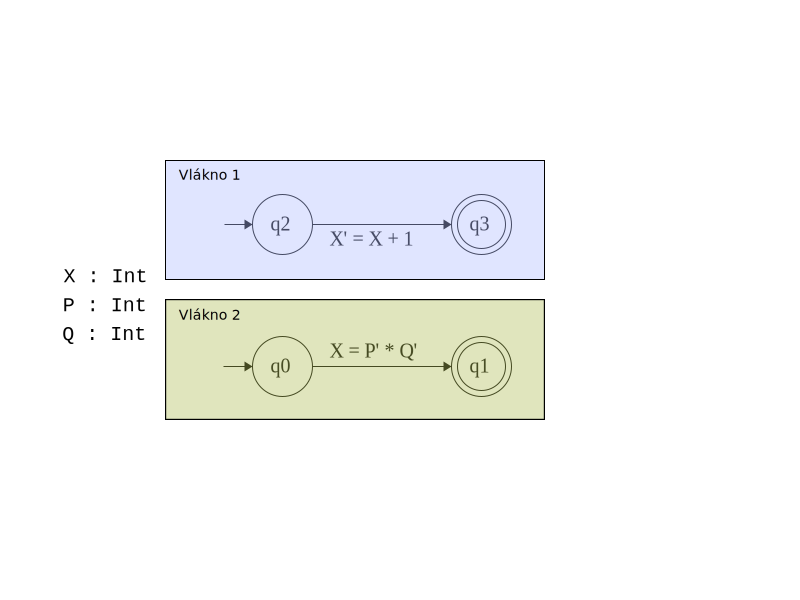
\includegraphics[scale=0.6]{transitionsystem.png}
\caption{Příklad přechodového systému}
\end{figure}
\begin{itemize}
\item Přechodový systém = konečný automat + proměnné
\item NTS - jazyk pro popis přechodových systémů
\item Předem daný počet vláken (a jejich kód)
\end{itemize}
\end{frame}



\begin{frame}{Přístup}
\begin{itemize}
\item Řešení = překlad + inlining + redukce
\item Vlastní reprezentace jazyka NTS (+ rozšíření)
\item Žádné předpoklady o vytváření vláken.
\item Omezená množina LLVM IR (bez pointerů, signed aritmetiky, \ldots)
\end{itemize}
\end{frame}

\begin{frame}{Paralelismus}
\begin{figure}
\includegraphics[width=0.8\textwidth]{paralelism.png}
\caption{Kód pracovního vlákna. Proměnná \texttt{F} obsahuje číslo funkce, která má běžet, a je nastavená voláním funkce \texttt{pthread\_create()}. }
\end{figure}
\end{frame}

\begin{frame}{Problémy}
\begin{itemize}
\item Rozdílný model paralelismu => méně efektivní redukce
\item Závislost na datech => zkoušení nemožných cest
\item Hrubé heuristiky => méně efektivní redukce
\end{itemize}
\end{frame}


\begin{frame}{Moje práce}
\begin{itemize}
\item Vybudování reprezentace NTS
\item Rozšíření NTS o datový typ BitVector.
\item Překlad podmožiny LLVM IR do NTS
\item Sekvencializace paralelního NTS (POR).
\end{itemize}
\end{frame}

\begin{frame}{Výsledky}
\begin{itemize}
\item Experimentů: málo
\item Redukovaný systém je zhruba poloviční (v počtu stavů i hran) oproti neredukovanému.
\item Hrubé aproximace, nízká efektivita.
\end{itemize}
\end{frame}

\begin{frame}{Možná rozšíření}
\begin{itemize}
\item Lepší heuristiky
\item Externí solver
\item Další části LLVM a Posix Threads
\end{itemize}
\end{frame}

\begin{frame}{Dotaz: vylepšení heuristiky pro C1}
\begin{question}
,,Je možné vylepšit heuristiku pro volbu A(Q) tak, aby nebylo nutné brát v potaz přechody z neaktivních úloh?''
\end{question}
\begin{itemize}
\item Úloha = vlákno v původním programu
\item C1: ,,Zvolíme - li jako A(Q) množinu povolených přechodů z vlákna P, pak nesmí existovat posloupnost přechodů mimo toto vlákno, z nichž některý by byl závislý na některém přechodu z A(Q).''
\item Jednoduchá heuristika: ,,žádné z ostatních vláken neobsahuje přechod závislý na přechodu z A(Q)''.
\item Problém: každé pracovní vlákno obsahuje přechody všech úloh.
\end{itemize}
\end{frame}


\begin{frame}{Dotaz: vylepšení heuristiky pro C1}
\begin{question}
,,Je možné vylepšit heuristiku pro volbu A(Q) tak, aby nebylo nutné brát v potaz přechody z neaktivních úloh?''
\end{question}
\begin{itemize}
\item Požadovaná heuristika: ,,žádná z ostatních aktivních úloh neobsahuje přechod závislý na některém přechodu z A(Q)''.
\item Stačí ukázat, že žádný běh mimo zvolené vlákno nemůže aktivovat novou úlohu.
\item Třeba vědět, kdy je úloha aktivována.
\item Speciální znalost: ,,Pro aktivaci úlohy je nutné zavolat funkci \texttt{thread\_create}''
\item Znalost dat: ,,Tato proměnná nikdy nenabude takovou hodnotu, aby byl přechod povolený.''
\end{itemize}
\end{frame}

\end{document}